\subsection{Choice of Fill Reducing Reordering}
\label{subseq:fill-in-reordering}

Fill reducing reordering is one of the first and the most important steps of sparse matrix factorization. As the name suggests, the step aims to reduce fill-in of $L$ and $U$ factors. However, it may have a strong and indirect impact on the elimination/assembly tree structure. As we discussed in subsection \ref{subseq:direct-parallel-aspects}, the structure defines tree-task parallelism as well as sizes of frontal matrices and, therefore, performance of the method.\\


MUMPS provides various algorithms for fill reducing reordering, as it was mentioned above. A detailed study and comparison of different methods were done by \citeauthor{guermouche2003memory}, in work \cite{guermouche2003memory}, for sequential execution of the analysis phase. \citeauthor{guermouche2003memory} noticed that  trees generated by METIS and SCOTCH were rather wide (because of the global partitioning performed at the top), while the trees generated by AMD, AMF and PORD tend to be deeper. In addition, they observed to two important things. Firstly, they noticed that both SCOTCH and METIS generated much better balanced trees in contrast to other methods. Secondly, according to their results, SCOTCH and METIS produced trees with bigger frontal matrices in contrast to those trees generated by other reordering techniques, \cite{guermouche2003memory}.\\


In this subsection, we are going to investigate influence of two different parallel fill reducing reordering algorithms provided by PT-Scotch and ParMETIS libraries on parallel performance of MUMPS. The algorithmic difference between the corresponding PT-Scotch and ParMETIS subroutines was mentioned in subsection \ref{subseq:mumps-review}.\\


To perform testing, PETSc, MUMPS, PT-Scotch and ParMETIS libraries were downloaded, compiled, configured and link together using their default settings. Tests were carried out using only flat-MPI mode on HW1 machine without any explicit process pinning. The results are shown in figure \ref{fig:mumps-ordering-1} as well as in appendix \ref{app:app-fill-reducing-reodering}.\\


\figpointer{\ref{fig:mumps-ordering-1}}
\begin{figure}[htpb]
\centering
	\begin{tabular}{cc}
		\subfloat[k3-18]{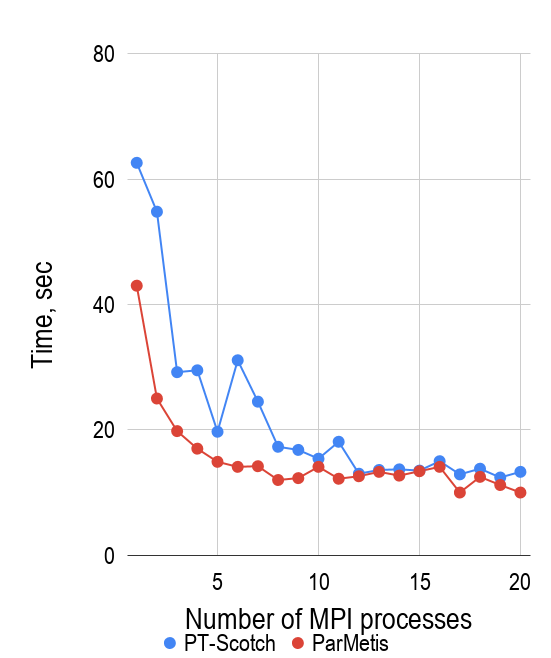
\includegraphics[width=0.48\textwidth]{figures/chapter-2/ordering/k3-18.png}} &
		\subfloat[cube-64]{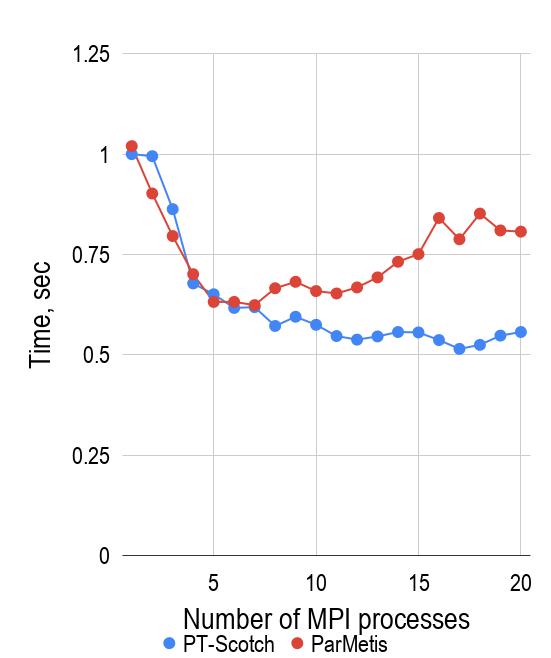
\includegraphics[width=0.48\textwidth]{figures/chapter-2/ordering/cube-64.png}} \\
		\subfloat[pwr-3d]{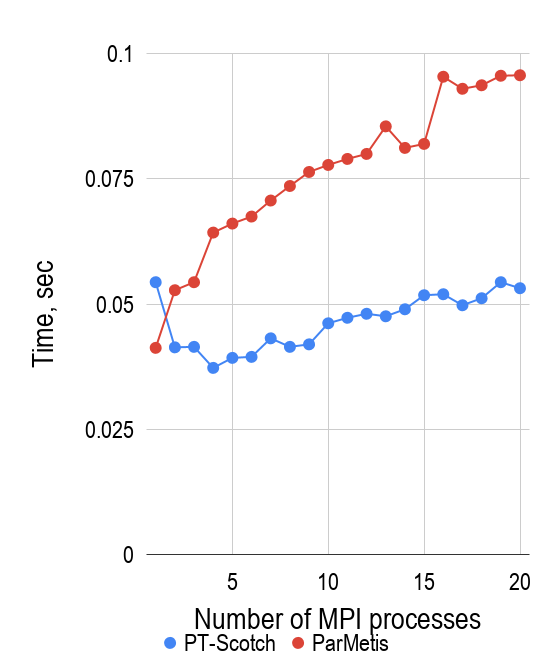
\includegraphics[width=0.48\textwidth]{figures/chapter-2/ordering/pwr-3d.png}} &
		\subfloat[k3-2]{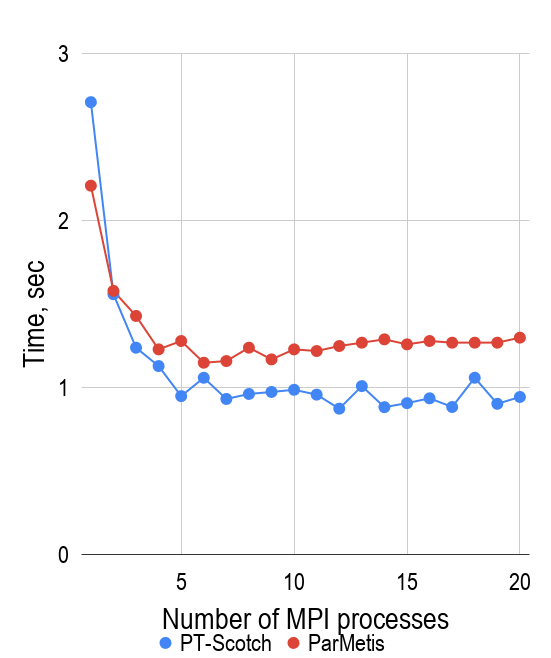
\includegraphics[width=0.48\textwidth]{figures/chapter-2/ordering/k3-2.png}} \\
	\end{tabular}
	\caption{Comparison of different fill-reducing algorithms}
	\label{fig:mumps-ordering-1}
\end{figure}



According to the results, parallel performance of MUMPS can vary significantly and very sensitive to a applied fill-in reducing reordering algorithm. In average, the difference between the algorithms achieves almost \textbf{15\%}. However, in some particular cases, \textit{cube-5} and \textit{pwr-3d}, the difference varies around \textbf{40-55\%}.\\


It is important to mention that both algorithms, PT-Scotch and ParMetis, are based on different heuristic approaches. It is relevant to assume that efficiency of a particular heuristic can be very sensitive to a matrix structure and size. This fact makes it difficult to predict in advance which algorithm is better to use for a specific case.\\


Considering results obtained with GRS matrix set, we can observe that PT-Scotch is the best choice for small and medium sized matrices, namely: \textit{cube-5}, \textit{cube-64}, \textit{k3-2} and \textit{pwr-3d} cases. Whereas, PerMetis tends to work better for relatively big systems, such as \textit{cube-645} and \textit{k3-18}, However, we keep in mind that number of GRS test-cases is not enough to make such conclusion and, therefore, the matrix set must be extended considerably for a future study.\\


% profiling of cube-5 and pwr-3d with ParMetis
During the test, we noticed that application of ParMetis to small systems of equations showed a strong negative effect on parallel performance of MUMPS. The results showed that factorization time of \textit{pwr-3d} and \textit{cube-5} matrices grew with the increase of the number of processing units, figure \ref{fig:mumps-ordering-matrices-total-time}.\\


\figpointer{\ref{fig:mumps-ordering-matrices-total-time}}
\begin{figure}[htpb]
\centering
	\begin{tabular}{cc}
		\subfloat[pwr-3d]{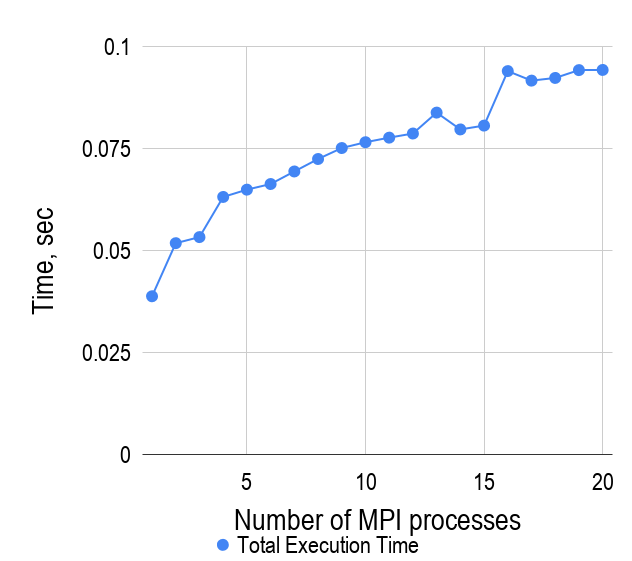
\includegraphics[width=0.475\textwidth]{figures/chapter-2/ordering/profiling/total-time-pwr-3d.png}} &
		\subfloat[cube-5]{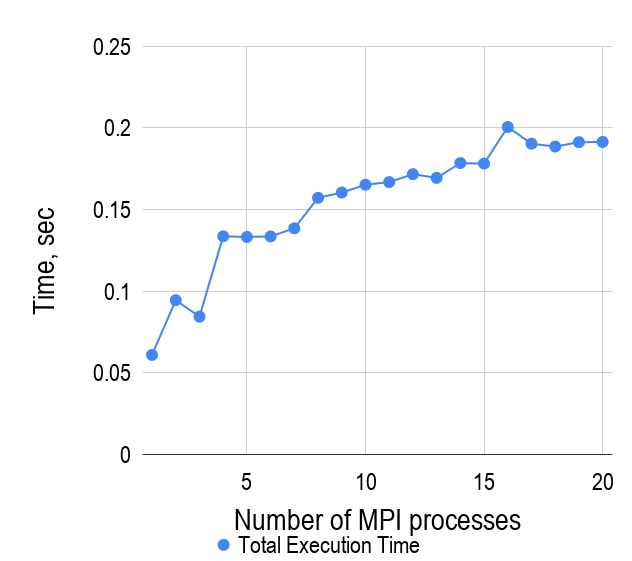
\includegraphics[width=0.475\textwidth]{figures/chapter-2/ordering/profiling/total-time-cube-5.png}} \\
	\end{tabular}
	\caption{MUMPS-ParMetis parallel performance in case of relatively small matrices}
	\label{fig:mumps-ordering-matrices-total-time}
\end{figure}


A simple profiling showed two important things. Firstly, numerical factorization time and time spent on the analysis phase had approximately the same order in case of sequential execution i.e. 1 MPI process. Secondly, while numerical factorization time were barely decreasing with increase of the number of processing elements, time spent on analysis phase significantly grew. Therefore, the slow-down of MUMPS in case of these two test-cases mainly came from overheads of the analysis phase.\\


A careful investigation revealed the analysis phase contained several peaks at points where the processor count was equal to a power of two. We assumed the cause could be due to either fill reducing reordering or process mapping steps. However, a detailed profiling and tracing of the analysis phase, which are out of the scope of this study, are required in order to give the exact answer. The results of profiling are shown in figure \ref{fig:mumps-ordering-matrices-profiling}.\\


\figpointer{\ref{fig:mumps-ordering-matrices-profiling}}
\begin{figure}[htpb]
\centering
	\begin{tabular}{cc}
		\subfloat[pwr-3d]{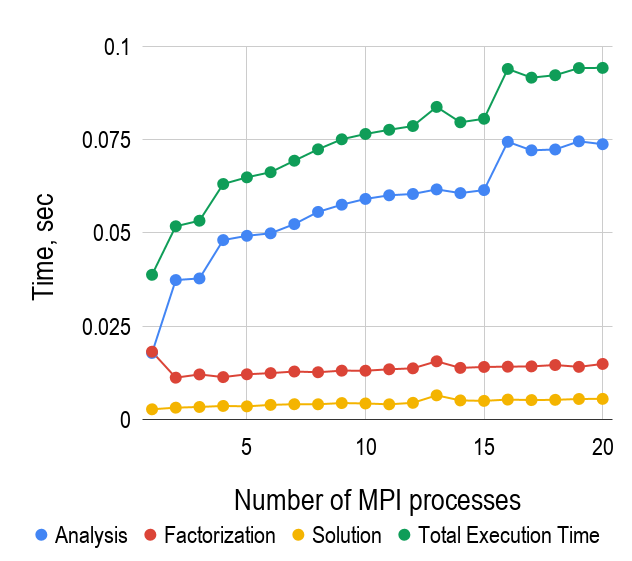
\includegraphics[width=0.475\textwidth]{figures/chapter-2/ordering/profiling/profiling-pwr-3d.png}} &
		\subfloat[cube-5]{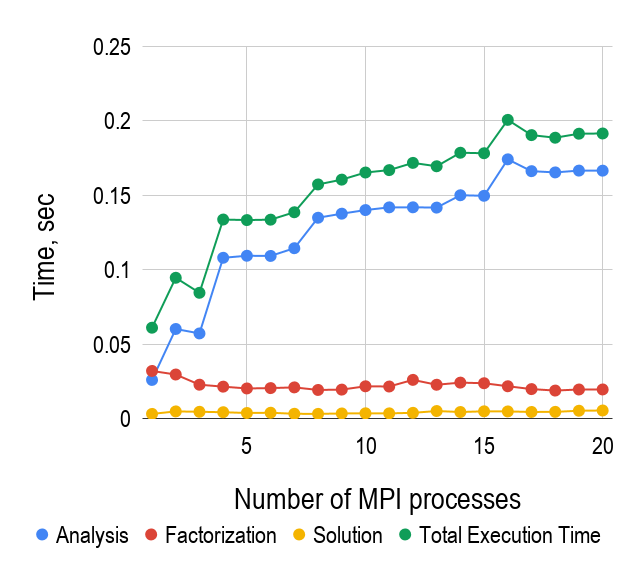
\includegraphics[width=0.475\textwidth]{figures/chapter-2/ordering/profiling/profiling-cube-5.png}} \\
	\end{tabular}
	\caption{Profiling of MUMPS library with using ParMetis as a fill-in reducing algorithm in case of factorization of relatively small matrices}
	\label{fig:mumps-ordering-matrices-profiling}
\end{figure}


\begin{table}[htpb]
\centering
\begin{tabular}{|c|c|c|c|c|}
\hline
Matrix Name & Ordering  & n       & nnz      & nnz / n \\ \hline
cube-5      & PT-Scotch & 9325    & 117897   & 12.6431 \\ \hline
cube-64     & PT-Scotch & 100657  & 1388993  & 13.7993 \\ \hline
cube-645    & ParMetis  & 1000045 & 13906057 & 13.9054 \\ \hline
k3-2        & PT-Scotch & 130101  & 787997   & 6.0568  \\ \hline
k3-18       & ParMetis  & 1155955 & 7204723  & 6.2327  \\ \hline
pwr-3d      & PT-Scotch & 6009    & 32537    & 5.4147  \\ \hline
\end{tabular}
\caption{GRS matrix set: assignment of matrices to a specific fill-in reducing algorithm based on parallel performance of flat-MPI tests}
\label{table:GRS-ordering-assignment}
\end{table}


In this subsection, we have presented the influence of  two different fill-in reducing algorithms on parallel performance of MUMPS. We have observed that a correct choice of an algorithm can lead to significant improvements in terms of the overall execution time. We have showed there is no a single algorithm that performs the best for all test-cases. At the moment of writing, we have come to a conclusion there is no an indirect metric to predict the best algorithm in advance for a specific system of equations. Sometimes PT-Scotch and ParMetis can result in nearly the same performance as it was, for example, in case of \textit{CurlCurl\_3} and \textit{cant} matrices, see appendix \ref{app:app-fill-reducing-reodering}. Therefore, from time to time, it can be quite difficult to decide which package to use even with available flat-MPI test results. At the end, we have assigned each test-case to a specific fill reducing reordering method based on results of the conducted experiments and our subjective opinion. The results are summarized it in tables \ref{table:GRS-ordering-assignment} and \ref{table:SuiteSparse-ordering-assignment}. \\ 


\begin{table}[htpb]
\centering
\begin{tabular}{|c|c|c|c|c|}
\hline
Matrix Name & Ordering  & n       & nnz      & nnz / n \\ \hline
cant        & ParMetis  & 62451   & 4007383  & 64.1684 \\ \hline
consph      & PT-Scotch & 83334   & 6010480  & 72.1252 \\ \hline
memchip     & PT-Scotch & 2707524 & 13343948 & 4.9285  \\ \hline
PFlow\_742  & PT-Scotch & 742793  & 37138461 & 49.9984 \\ \hline
pkustk10    & PT-Scotch & 80676   & 4308984  & 53.4110 \\ \hline
torso3      & ParMetis  & 259156  & 4429042  & 17.0903 \\ \hline
x104        & PT-Scotch & 108384  & 8713602  & 80.3956 \\ \hline
CurlCurl\_3 & PT-Scotch & 1219574 & 13544618 & 11.1060 \\ \hline
Geo\_1438   & ParMetis  & 1437960 & 63156690 & 43.9210 \\ \hline
\end{tabular}
\caption{SuiteSparse matrix set: assignment of matrices to a specific fill-in reducing algorithm based on parallel performance of flat-MPI tests}
\label{table:SuiteSparse-ordering-assignment}
\end{table}


From now onwards, assignments mentioned in tables \ref{table:GRS-ordering-assignment}, \ref{table:SuiteSparse-ordering-assignment} is going to be used without explicitly referring to it.\\